\documentclass[12pt]{article}
\usepackage{amsmath,amsfonts,nicefrac}
\usepackage{graphicx}
\usepackage{enumerate}
\usepackage{natbib}
\usepackage{url} % not crucial - just used below for the URL 
\usepackage{ifthen}

%\pdfminorversion=4
% NOTE: To produce blinded version, replace "0" with "1" below.
\newcommand{\blind}{1}
% DON'T change margins - should be 1 inch all around.
\addtolength{\oddsidemargin}{-.5in}%
\addtolength{\evensidemargin}{-.5in}%
\addtolength{\textwidth}{1in}%
\addtolength{\textheight}{-.3in}%
\addtolength{\topmargin}{-.8in}%


\usepackage[table]{xcolor}% http://ctan.org/pkg/xcolor

\newcommand{\cl}[2]{\cellcolor{#1!#2}}
\newcommand{\inc}[2]{ \ifthenelse{\equal{#1}{1}}{\input{./sections/#2}}{ } }



\begin{document}

%\bibliographystyle{natbib}

\def\spacingset#1{\renewcommand{\baselinestretch}%
{#1}\small\normalsize} \spacingset{1}


%%%%%%%%%%%%%%%%%%%%%%%%%%%%%%%%%%%%%%%%%%%%%%%%%%%%%%%%%%%%%%%%%%%%%%%%%%%%%%

\if1\blind
{
  \title{\bf Towards Structured Use of Bayesian Sequential Monitoring in Clinical Trials}
  \author{Evan Kwiatkowski\textsuperscript{$\dagger$}, 
	        Eugenio Andraca-Carrera\textsuperscript{$\ddagger$},\\
					Mat Soukup\textsuperscript{$\ddagger$},
					\medskip Matthew A. Psioda\textsuperscript{$\dagger$}\thanks{The authors gratefully acknowledge \textit{please remember to list all relevant funding sources in the unblinded version}}\\
	  %
	  $\dagger$ Department of Biostatistics,
		University of North Carolina, \\
		McGavran-Greenberg Hall, CB\#7420, \\
		%
		\medskip Chapel Hill, North Carolina, U.S.A.\\
    $\ddagger$ Division of Biometrics VII, Office of Biostatistics \\
		           Center for Drug Evaluation and Research, \\
							 US Food and Drug Administration, \\
							 Silver Spring, Maryland, USA \\									
		}
  \maketitle
} \fi

\if0\blind
{
  \bigskip
  \bigskip
  \bigskip
  \begin{center}
    {\LARGE\bf Title}
\end{center}
  \medskip
} \fi

\bigskip
\begin{abstract}
The text of your abstract. 200 or fewer words.
\end{abstract}

\noindent%
{\it Keywords:}  3 to 6 keywords, that do not appear in the title
\vfill

\newpage
\spacingset{1.5} % DON'T change the spacing!



\section{Introduction}

Things to discuss:
\begin{itemize}
 \item 21\textsuperscript{st} Century Cures Act (MATT)
 \item PDUFA VI reauthorization (MATT)
 \item Expansive work already done on sequential monitoring  (EVAN -- draft on 6/21)
%\item Berry A Case for Bayesianism, Cornfield The Bayesian outlook, classical arguments for Bayes in clinical trials, not sequential monitoring in particular
%\item (1) Berry Montoring Accumulating Data, (2) Cornfield/Greenhouse On certain aspects, (3) Cornfield Sequential Trials, (4) A Bayesian Test of Some Classical Hypotheses, with Applications to Sequential Clinical Trials Jerome Cornfield 
%\item Bayes \& monitoring, based on posterior distributions
%\item First papers in Bayes sequential monitoring. Bayesian inferences not affected by frequent or continual monitoring by the likelihood principle.
%\item Papers which compare to frequentist stopping rules \& increased interpretation on role of priors.
%\item \cite{Spiegelhalter1994}
%\item \cite{Spiegelhalter1993} predictive distributions as basis for monitoring
%\item \cite{Freedman1992} choice of prior explained by showing its impact on percentiles of posterior distribution
%\item \cite{Freedman1989} The need to overcome this `\textbf{handicap}' prevents unduly early termination.
%\item \cite{Fayers1997} Choosing these two priors (skeptical, enthuastic) provides a useful \textbf{brake} against the premature termination of trials.
%\item Bayesian Adaptive Methods for Clinical Trials Berry, Carlin, Etc.
 \item Our majors contribution (EVAN -- as early as possible in introduction without having the flow appear weird -- draft on 6/21)
 \item Outline for the remaining section of the paper (EVAN -- draft on 6/21)
\end{itemize}
The theoretical foundations for the Bayesian clinical trials has been long established \cite{Cornfield1966}~\cite{Cornfield1966a}~\cite{Neyman1967}. These methods were not widely used in practice until a comprehensive framework for interpretation of results was developed through specifying prior distributions that were naturally and intuitively related to the research objectives (e.g. skeptical and enthuastic priors) \cite{Freedman1989}~\cite{Freedman1992}~\cite{Spiegelhalter1993}~\cite{Spiegelhalter1994}~\cite{Fayers1997}. (\textit{Rewrite paragraph.})

There is still potential for further utilization of Bayesian methods in the clinical trial setting. While the framework for interpretation of Bayesian clincial trials is well devloped, the details of specifying prior distributions in a natural and intuitive way is lacking. This paper presents a structured or default way to determine prior distributions based on the trial design. Our major contribution is to present methods for the default or automatic selection of prior distributions in a way that is applicable to a wide array of clinical trial designs.

\begin{enumerate}
\item Bayesian methodology is widely developed.
\item It has been applied (cite).
\item The current perspective is that Bayesian methodology is only valid when Frequentist methods are insufficient, including where enrollment is challenging (rare diseases, pediatric studies)
\item Our contribution is to show that Bayesian methods are applicable to all clinical trials. This is shown by highlighting their improved interpretation and showing their use in varied and complicated situations.
\end{enumerate}

\section{Methods}

As you introduce ideas that come from or extend other ideas in the literature, cite the relevant literature.

\subsection{Monitoring versus Estimation Priors}

%\begin{itemize}
% \item Define generally in terms of $\boldsymbol\theta = \left( \gamma, \boldsymbol\psi  \right)$ where $\gamma$ is a parameter of interest
%       and $\boldsymbol\psi$ is a nuisance parameter (possible vector valued).
% \item Define \textit{Monitoring} Priors and \textit{Inference} Priors.
% \item Make connection between Inference priors and two-part mixture prior and BMA.
% \item Define \textit{Skeptical} and \textit{Enthusiastic} monitoring priors and how each would be used.
% \item I would have a generic graphic to illustrate the types of priors and the mixture.
% %\item Motivate in the context of a simple example (i.e., single parameter binary example).
%\end{itemize}

\subsubsection{Bayesian hypothesis testing based on posterior probabilities}

The Bayesian paradigm provides direct inference on a parameter of interest through specification of a model for the data generating mechanism and prior distributions for unknown quantities. Let $\mathbf{D}$ be a random variable representing the data collected in the trial with density $p(\mathbf{D}|\theta,\psi)$ where $\theta$ and $\psi$ are the unknown quantities. Let $\theta$ be the parameter of interest and $\psi$ be the unknown quantities that are not of primary importance (nuisance parameters). Define the sample spaces for the unknown quantities as $\theta\in\Theta$ and $\psi\in\Psi$. 

Suppose the hypothesis for the trial is $H_0:\theta\in\Theta_0$ versus $H_1:\theta\in\Theta_1$. These hypotheses are judged based on posterior probabilities of $\theta$ by evaluating its marginal likelihood 
\begin{align*}
P(\theta\in\Theta_i|\mathbf{D})=\int_{\Theta_i}p(\theta|\mathbf{D})d\theta\text{ for }i\in\{0,1\},
\end{align*}
where $p(\theta|\mathbf{D})=\int_{\Psi}p(\theta,\psi|\mathbf{D})d\psi$ is marginalized over the nuisance parameters.

\subsubsection{Prior elicitation}
It has been said that ``the purpose of a trial is to collect data that bring to conclusive consensus at termination opinions that had been diverse and indecisive at the \textit{outset}" (Kass and Greenhouse (1989), emphasis added). These opinions manifest as priors $\pi(\theta,\psi)$ for which their relation to $P(\theta\in\Theta_i|\pi(\theta,\psi))$ $i\in\{0,1\}$ is examined. Note this quantity does not depend on the data $\mathbf{D}$ and therefore reflects a-priori opinion.

The posterior distribution of $\theta$ depends on the choice of prior distribution $\pi(\theta,\psi)$ since $p(\theta,\psi|\mathbf{D})=p(\mathbf{D}|\theta,\psi)\pi(\theta,\psi)/p(\mathbf{D})$ by Bayes rule. The specification of the prior distribution depends on the research objective. An \textit{inference prior} is a prior that is used when the research objective is to make final analysis after data collection is complete. A \textit{monitoring prior} is a prior that is used when the research objective is to see if there is a persuasive result based in the interim data. Stopping for efficacy is ceasing enrollment due to a promising interim result (one that is consistent with $H_1$, and stopping for futility is ceasing enrollment due to a discouraging interim result (one that is consistent with $H_0$).

Define $\delta\in(0,1)$ as a threshold for \textit{a compelling level of evidence} as it relates to $\theta$. We say that an individual is ``all but convinced" that $H_i$ is true given the observed data if $P(\theta\in\Theta_i|\mathbf{D})\geq\delta$ for $i\in\{0,1\}$. The quantity $1-\delta$ reflects \textit{residual uncertainty} of $H_i$ being true relative to the competing hypothesis. %For example, an individual would be ``all but convinced" of the truth of the alternative hypothesis if $P(\theta\in\Theta_1|\mathbf{D})\geq\delta$.


%Possible simplifying functional relationships between $\theta$ and $\psi$ are conditional independence $\pi(\theta,\psi)=\pi(\theta|\psi)\pi(\psi)$ and independence $\pi(\theta,\psi)=\pi(\theta)\pi(\psi)$. An inference prior is often non-informative or objective in the sense that it does not show preference to $H_0$ or $H_1$. Decisions made using using a non-informative prior are often similar to those made in the frequentist setting. 
A enthuastic prior is an informative prior that gives preference to $H_1$ such that it is ``all but convinced" that $H_1$ is true a-priori. This prior $\pi_{E}(\theta,\psi)\equiv\pi_{E}$ has the property that $P(\theta\in\Theta_1| \pi_{E})\geq\delta$ (equivalently $P(\theta\in\Theta_0| \pi_{E})<1-\delta$). The choice of $\delta\in(0,1)$ is motivated by \textit{a compelling level of evidence} as it relates to $\theta$, although in this setting the ``evidence" reflects a theoretical opinion rather than empirical judgement. For example, if $\delta=0.95$, then this choice of enthaustic prior places 95\% prior probability that $\theta\in\Theta_1$.  

A skeptical prior is an informative prior that does not give strong preference to $H_1$. This prior $\pi_{S}(\theta,\psi)\equiv\pi_{S}$ could have the property that $P(\theta\in\Theta_0| \pi_{S})\geq\delta$, in which case it is ``all but convinced" that $H_0$ is true a-prior, however, this demonstrates such an extreme disbelief in the possibility of a positive effect that conducting the trial at all would be viewed as dubious. Consider a region $\Theta_A\subset\Theta_1$ that demonstrates a sizeable positive effect. The skeptical prior is then constructed such that $P(\theta\in\Theta_A| \pi_{S})<\delta$.

\subsubsection{Sequential monitoring}
The use of monitoring based on changing the opinion of skeptical and enthuastic priors has been described as overcoming a handicap (\cite{Freedman1989}) and providing a brake (\cite{Fayers1997}) on the premature termination of trials, or constructing ``an adversary who will need to be disillusioned by the data to stop further experimentation" (\cite{Spiegelhalter1994}). Early termination of enrollment is appriopriate if diverse prior opinions about $\theta$ would be in agreement given the interim data (e.g. the skeptical and enthuastic person reach the same conclusion). 

\subsubsection*{Promising interim result}
In order for interim evidence showing $H_1$ is true to be persuasive, it has to cause the skeptic, who initially held that $P(\theta\in\tilde{\Theta}\subset\Theta_1| \pi_{S})<\delta$, to believe that $P(\theta\in\Theta_1| \pi_{S})\geq\delta$.
\subsubsection*{Disillusioning interim result}
In order for interim evidence showing $H_1$ is false to be persuasive, it has to cause the enthusiast, who initially held that $P(\theta\in\Theta_1| \pi_{E})\geq\delta$, to believe that $P(\theta\in\tilde{\Theta}\subset\Theta_1| \pi_{E})<\delta$

\subsubsection*{Example}
\begin{figure}
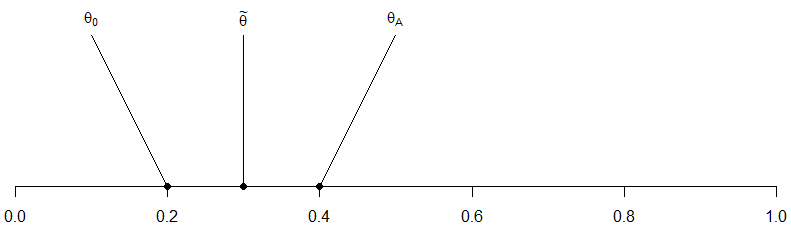
\includegraphics[width=6in]{D:/Users/ekwiatko/Documents/GitHub/Bayesian-Sequential-Monitoring/00-paper/FIGURES/line_graph}
\caption{}
\end{figure}

Consider the hypothesis $H_0:\theta\leq\theta_0$ vs. $H_1:\theta>\theta_0$. The skeptic initially held that $P(\theta>\theta_A| \pi_{S})<\delta$ and a promising interim result would be $P(\theta>\theta_0| \pi_{S})\geq\delta$. The enthusiast initially held that $P(\theta>\theta_0| \pi_{E})\geq\delta$ and a disillusioning interim result would be $P(\theta>\tilde{\theta}| \pi_{E})<\delta$

\subsubsection*{Probability of Success}
%Summarizing~\cite{Spiegelhalter1993} and others:  or that the benefit of treatment is not likely to be what was expected, the probability of \textit{eventually} proving that $H_1$ is true is sufficiently low, or the resources have been exhausted.  
%A standard Bayesian decision rule would reject $H_0$ when $P(\theta\in\Theta_{H_1}|D\geq 0.95)$ which will result in a Type I error rate of $0.05$ when the analysis prior is non-informative (a so-called reference or flat prior). The Bayes factor in favor of $H_0$ is defined as 
%\begin{align*}
%BF=\frac{p(D|H_0)}{p(D|H_1)}=\frac{\int_{\Theta_{H_0}}p(D|\theta,H_0)\pi(\theta|H_0)d\theta}{\int_{\Theta_{H_1}}p(D|\theta,H_0)\pi(\theta|H_1)d\theta}
%\end{align*}
%and let $p(\theta|D,\pi)$ denote the posterior distribution of $\theta$ given a particular prior distribution.
As an alternative strategy to futility analysis, one can monitor the probability of success (POS) for the trial. The probability of getting a convincing result at the end of the trail can be computed using the interim data. Let $p(\theta|\mathbf{D}, \pi_{I})$ denote the posterior distribution for $\theta$ based on the inference prior $ \pi_{I}$ and the current data $\mathbf{D}$. Let $\xi$ denote the POS which is given as follows:
\begin{align*}
\xi&=P[\mathbf{D}_1\in\mathbb{R}^{dim(\mathbf{D}_1)}|P(\theta\in\Theta_1|\mathbf{D}_1,\mathbf{D},\pi_I)\geq\delta]\\
&=E[1\{P(\theta\in\Theta_1|\mathbf{D}_1,\mathbf{D}, \pi_{I})\geq \delta\}]
\end{align*}
where the expectation is taken with respect to the posterior predictive distribution $p(\mathbf{D}_1)$ for future data $\mathbf{D}_1$ (which includes subjects yet to enroll):
\begin{align*}
p(\mathbf{D}_1)=\int p(\mathbf{D}_1|\theta)\cdot \pi(\theta|\mathbf{D})d\theta.
\end{align*}
One may stop the enrollment if $\xi$ is sufficiently small (i.e. $\xi<0.05$).
\subsubsection{Final inference}
Final inference on the parameter of interest is made once all data has been collected. Enrollment was either stopped based on a persuasive interim result or based on the maximum sample size. An inference prior $\pi_{I}(\theta,\psi)\equiv\pi_{I}$ is often less divisive than the skeptical and enthaustic priors, and can be viewed as a balance of the more divisive opinions. We propose use of a mixture prior constructed from the monitoring process as the inference prior:
\begin{align*}
\pi_{I}=\omega\cdot\pi_{S}+(1-\omega)\cdot\pi_E
\end{align*}
for $\omega\in[0,1]$. Choosing $\omega=1/2$ for an equal mixture of $\pi_S$ and $\pi_E$ corresponds to an inference prior that equally weights the skeptical and enthuastic opinions. Define $p(\mathbf{D}|\pi(\theta,\psi))=\int p(\mathbf{D}|\theta)\pi(\theta,\psi)d(\theta,\psi)$ to be the marginal likelihood for the data given the prior $\pi(\theta,\psi)$. Choosing $\omega$ based on posterior model probabilities of the null and alternative hypotheses yields $\omega=p(\mathbf{D}| \pi_{S})/(p(\mathbf{D}| \pi_{S})+p(\mathbf{D}| \pi_{E}))$. 

%The determination of a significant trial result is given by
%\begin{align*}
%P(\theta\in\Theta_1|\mathbf{D},\pi_I)\geq\delta.
%\end{align*} 

All relevant information about $\theta$ can be derived from its marginal posterior distribution with an inference prior (e.g. posterior mean, credible intervals). For example, the posterior mean using the inference prior will be a two-part mixture of the posterior means using the skeptical and enthuastic priors:
\begin{align*}
E(\theta|\mathbf{D},\pi_I)&=\omega\cdot E(\theta|\mathbf{D}, \pi_{S})+(1-\omega)\cdot E(\theta|\mathbf{D}, \pi_{E})%\\
%\int_\Theta \theta p(\theta|\mathbf{D},\pi_{I})d\theta&=\omega\cdot \int_\Theta \theta p(\theta|\mathbf{D},\pi_{S})d\theta+(1-\omega)\cdot\int_\Theta \theta %p(\theta|\mathbf{D},\pi_{E})d\theta
\end{align*}
%\begin{align*}
%\pi_{Inference}=\frac{p(\mathbf{D}| \pi_{S}) \pi_{S}+p(\mathbf{D}| \pi_{E}) \pi_{E}}{p(\mathbf{D}| \pi_{S})+p(\mathbf{D}| \pi_{E})}
%\end{align*}
%\begin{align*}
%E(\theta|\mathbf{D},\pi_{Inference})=\omega\times E(\theta|\mathbf{D}, \pi_{S})+(1-\omega)\times E(\theta|\mathbf{D}, \pi_{E})
%\end{align*}
%Need to describe relation to Type I and Type II error.
%\subsubsection{Default parameterization of monitoring priors for common designs}\label{monitoring_prior_specification}
%Define prior distribution as $\pi(\theta|\lambda)$ where $\lambda$ is a vector of hyperparameters.

%Reference prior attempts to express no particular opinion about the treatment's merit. 



%\subsection{Futility Monitoring Using Probability of Success (EVAN -- draft on 6/21)}
%
%\begin{itemize}
% \item Futility monitoring using POS is about stopping early when their is a high likelihood
%       of a study being inconclusive at the end of the study.
% \item Since the final analysis uses the \textit{Inference} prior, POS should be based on the
%       inference prior.
% \item Develop the framework for POS and show how it is a weighted average POS based on the skeptical
%       and enthusiastic priors.
%\end{itemize}


%Stochastic curtailment in frequentist setting.
\section{Examples}

\subsection{Single-Arm Proof-of-Activity Trial with Binary Endpoint}

\subsubsection{Model formulation \& prior elicitation}

Consider a single-arm oncology proof-of-activity trial with a binary endpoint. The data $\mathbf{D}$ are Binomially distributed and the response rate $\theta$ is the parameter of interest, with higher values of $\theta$ being indicative of proof-of-activity. The formulation is discussed in (cite example) with $\theta_0=0.2$, $\tilde{\theta}=0.3$, $\theta_A=0.4$.

It is intuitive to center the skeptical and enthuastic priors around the quantities $\theta_0$ and $\theta_A$ respectively, so that $E(\pi_S)=\theta_0$ and $E(\pi_E)=\theta_A$.

Beta priors for $\theta$ will be used to provide closed-form expressions of the posterior distributions via Beta-Binomial conjugacy (the posterior distribution $p(\theta|\mathbf{D})$ will be Beta distributed). In particular, let $y_1$ be the number of successes and $y_0$ be the number of failures. If the skeptical prior is $\pi_S(\theta)\sim\mathcal{B}(\alpha_S,\beta_S)$ then the associated posterior is $p(\theta|\mathbf{D},\pi_S)\sim\mathcal{B}(\alpha_S+y_1,\beta_S+y_0)$. Similarly, if the enthuastic prior is $\pi_E(\theta)\sim\mathcal{B}(\alpha_E,\beta_E)$ then the associated posterior is $p(\theta|\mathbf{D},\pi_E)\sim\mathcal{B}(\alpha_E+y_1,\beta_E+y_0)$.

The skeptical prior is Beta distributed with expected value $\theta_0=0.2$ and has $4.5\%$ prior probability that $\theta>\theta_A=0.4$. The enthuastic prior has expected value $\theta_A=0.4$ and has $5\%$ prior probability that $\theta<\theta_0=0.2$. The inference prior will be at an equal mixture of the skeptical and enthuastic prior ($\omega=0.5)$.
\begin{figure}
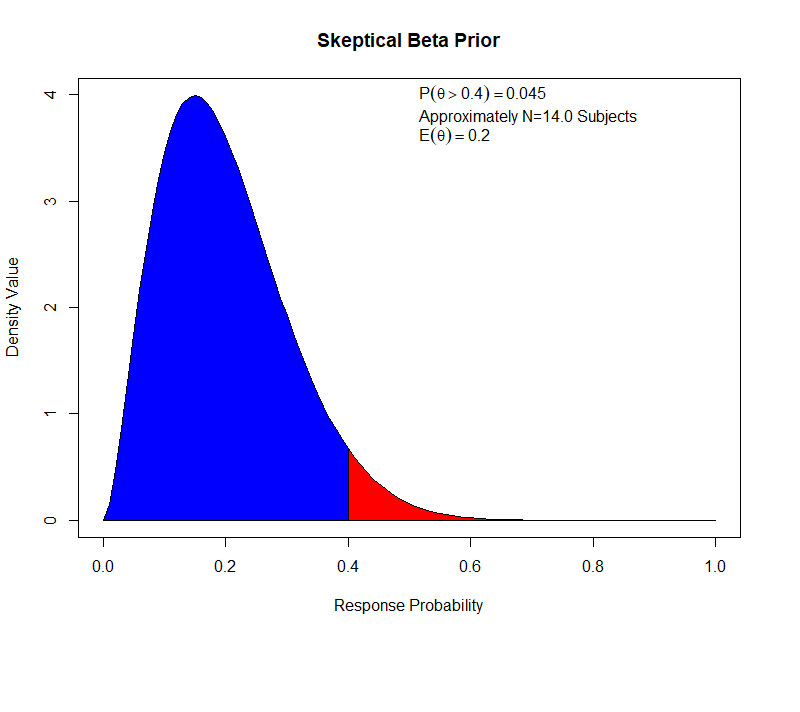
\includegraphics[width=3in]{D:/Users/ekwiatko/Documents/GitHub/Bayesian-Sequential-Monitoring/00-paper/FIGURES/skpt_prior}
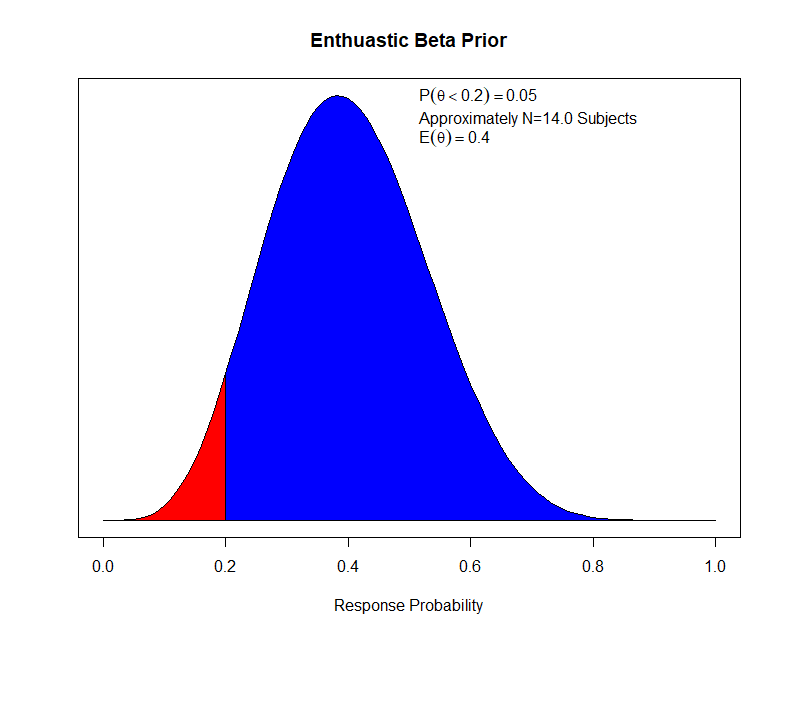
\includegraphics[width=3in]{D:/Users/ekwiatko/Documents/GitHub/Bayesian-Sequential-Monitoring/00-paper/FIGURES/enth_prior}
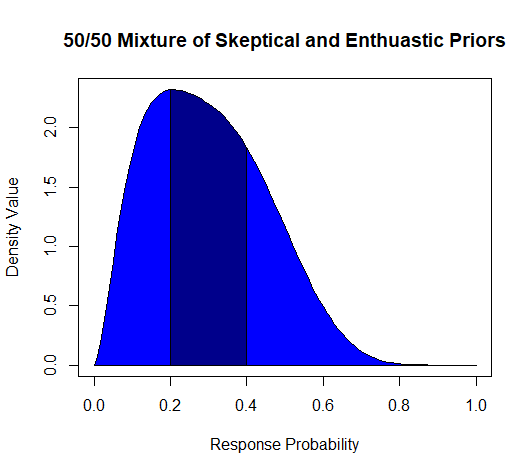
\includegraphics[width=3in]{D:/Users/ekwiatko/Documents/GitHub/Bayesian-Sequential-Monitoring/00-paper/FIGURES/5050mix}
\caption{(a) Skeptical prior (b) Enthuastic prior (c) 50/50 mixture of skeptical and enthuastic prior}
\end{figure}

\newpage
\subsubsection{Sequential monitoring}
The trial will proceed until one of the following three conditions are satisfied:
\begin{align*}
\text{Efficacy criteria: }&P(\theta>0.20|\mathbf{D},\pi_S)\geq 0.95\\
\text{Futility criteria: }&P(\theta\leq 0.30|\mathbf{D},\pi_E)\geq 0.85\\
\text{Maximum sample size: }&N=76 \text{ patient outcomes obtained}
\end{align*}
The maximum sample size is based on a frequentist design that would have $90\%$ power at 0.35.


%\begin{center}
%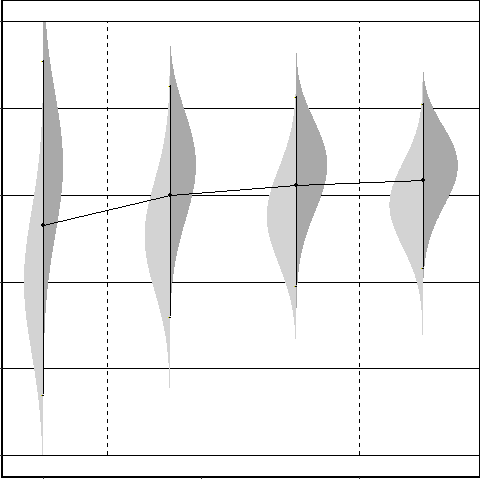
\includegraphics[width=5in]{D:/Users/ekwiatko/Documents/GitHub/Bayesian-Sequential-Monitoring/00-paper/FIGURES/violin_efficacy.png}
%\end{center}
%\begin{center}
%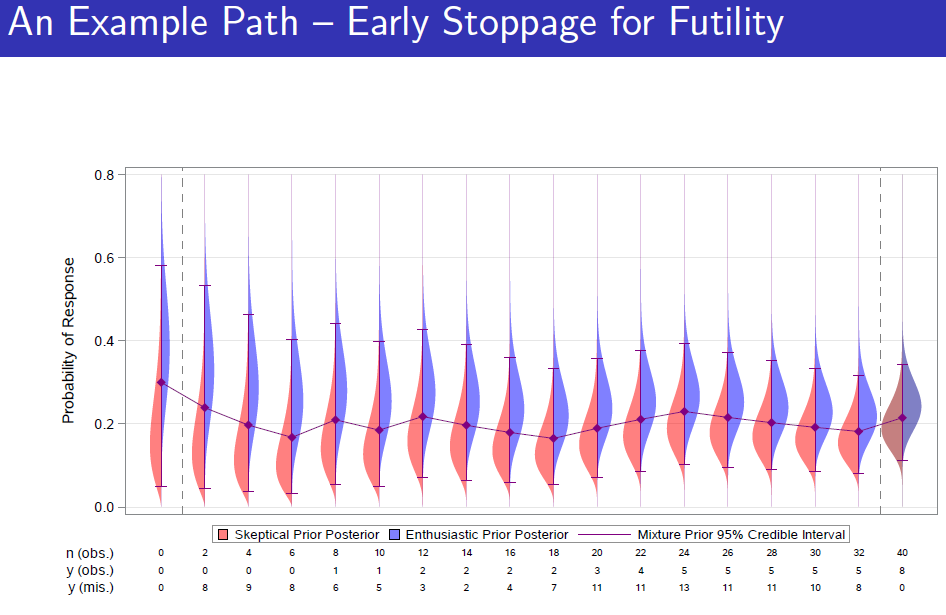
\includegraphics[width=5in]{D:/Users/ekwiatko/Documents/GitHub/Bayesian-Sequential-Monitoring/00-paper/FIGURES/violin_futility.png}
%\end{center}
\newpage
\subsubsection{Example paths}
As seen in Figure 3(a), at the second interim analysis the efficacy condition $P(\theta>0.20|\mathbf{D},\pi_S)\geq 0.95$ is satisfied and enrollment is terminated. As shown in Figure 3(b), at the fourth interim analysis the futility condition $P(\theta\leq 0.30|\mathbf{D},\pi_E)\geq 0.85$ is satisfied and enrollment is terminated.
\begin{figure}
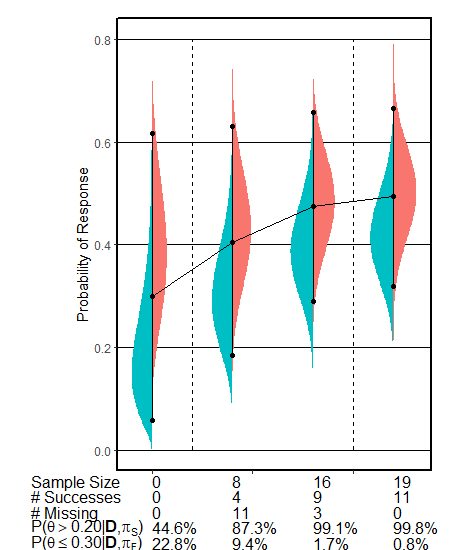
\includegraphics[width=3.5in]{D:/Users/ekwiatko/Documents/GitHub/Bayesian-Sequential-Monitoring/00-paper/FIGURES/violin_efficacy_ekk.png}
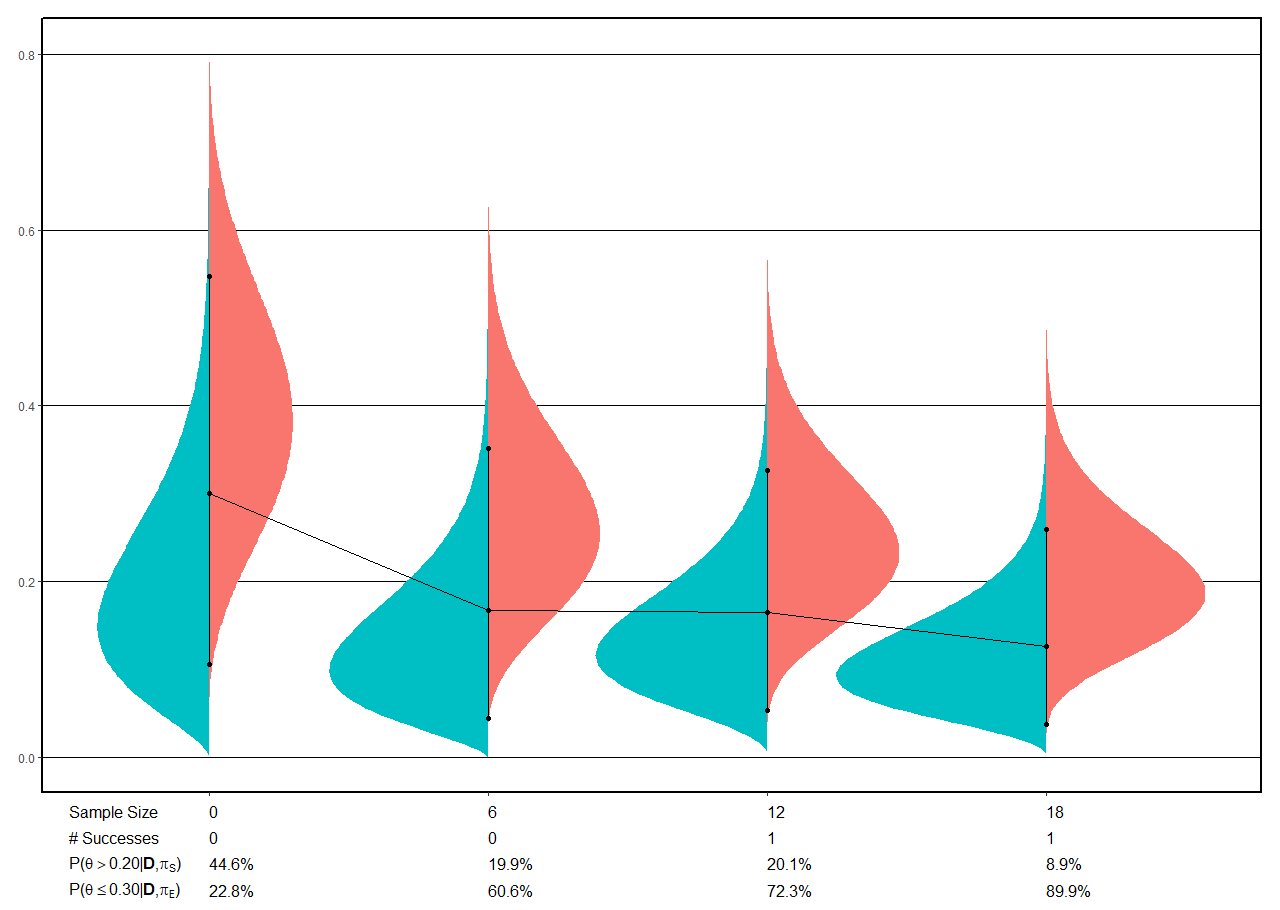
\includegraphics[width=3.5in]{D:/Users/ekwiatko/Documents/GitHub/Bayesian-Sequential-Monitoring/00-paper/FIGURES/violin_futility_ekk.png}
\caption{(a) Early stopping for efficacy (b) Early stopping for futility}
\end{figure}
\newpage
\subsubsection{Design properties: Results}
Assume that the outcomes are ascertained after approximately 4 months of follow-up and 2 patients per month on average are enrolled. An interim analysis will be completed after every 2 subjects complete follow-up.
\begin{figure}
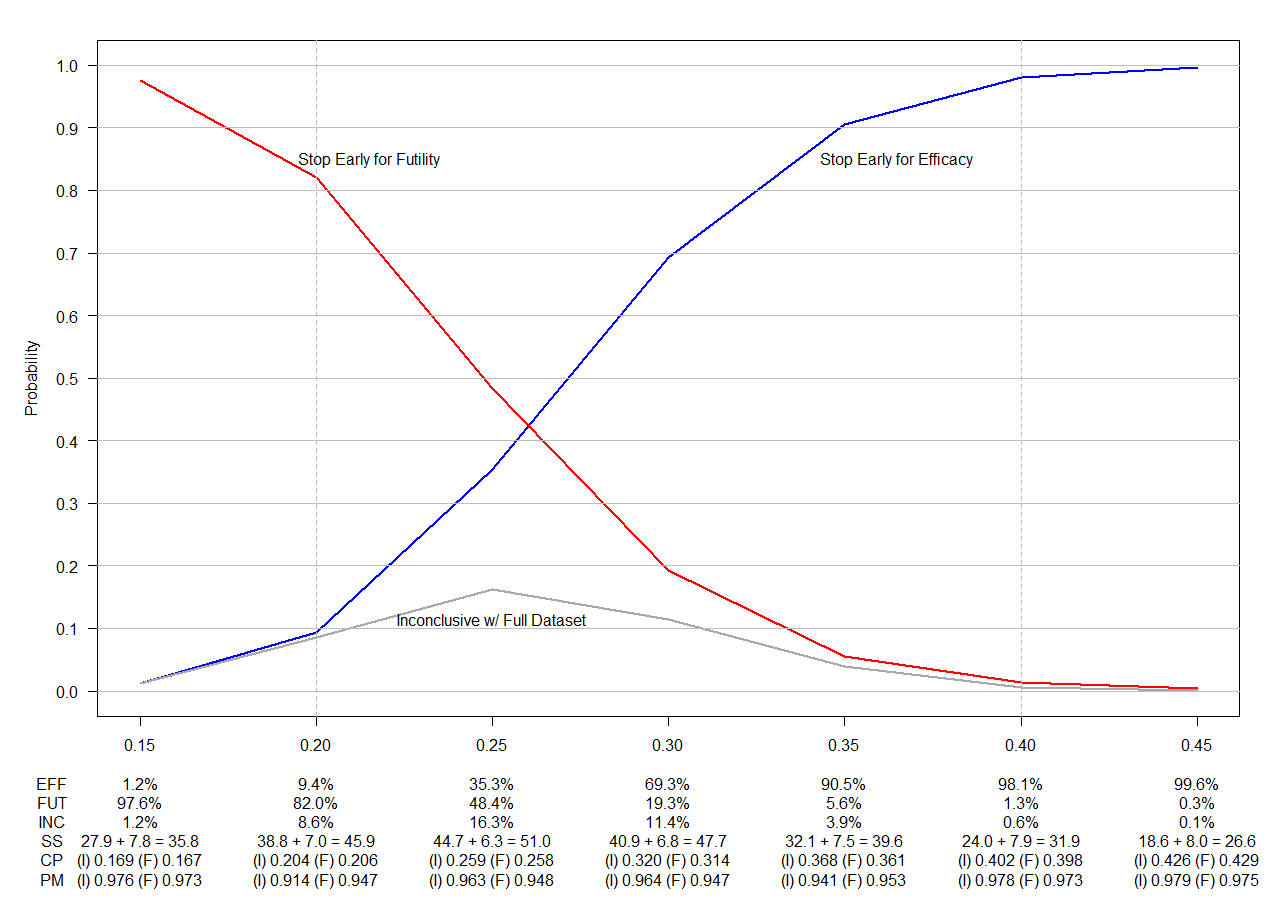
\includegraphics[width=7in]{D:/Users/ekwiatko/Documents/GitHub/Bayesian-Sequential-Monitoring/00-paper/FIGURES/seq_des_pro}
\caption{}
\end{figure}
Let EFF be the probability of the trial stopping early for efficacy, FUT be the probability of the trial stopping early for futility, and INC be the probability of reaching the maximum sample size without a conclusive monitoring result. Let SS be the average sample size at the definitive interim analysis (I) and at the end of follow-up (F), let CP be the coverage probability using the mixture prior, and let PM be the posterior mean an inference prior which is a 50/50 mixture of the skeptical and enthuastic priors.
\newpage
\subsubsection{Agreement between interim and final result}
\begin{center}
\textbf{Distribution of final posterior probability given interim stoppage (interim $P(\theta>0.20|\mathbf{D},\pi_S)\geq 0.95$) and evidence decrease.}
\begin{tabular}{l|ccccccc}
&0.15&0.20&0.25&0.30&0.35&0.40&0.45\\
\hline
Final $P(\theta>0.20|\mathbf{D},\pi_S)\geq 0.95$ &29.3\%&51.0\%&64.5\%&75.3\%&83.2\%&89.4\%&93.2\% \\ 
Final $P(\theta>0.20|\mathbf{D},\pi_S)< 0.95$&70.7\%&49.0\%&35.5\%&24.7\%&16.8\%&10.6\%&6.8\%\\  
\hspace{0.5in}Conditional Median&0.91&0.92&0.92&0.93&0.93&0.93&0.93\\  
\hspace{0.5in}Conditional 25th percentile&0.87&0.89&0.90&0.91&0.91&0.91&0.91\\  
\hspace{0.5in}Conditional 10th percentile&0.83&0.86&0.87&0.88&0.88&0.88&0.88\\  
\hspace{0.5in}Conditional 1st percentile&0.67&0.78&0.81&0.81&0.82&0.82&0.82
\end{tabular}
\end{center}

For example, at a true response rate of $\theta=0.40$, there is an $89.4\%$ that the threshold for a significant result is maintained after the additional subjects complete follow-up, and in the $10.6\%$ of cases that the evidence decreases, the median posterior probability is $0.93$ and only in $10\%$ of cases is the posterior probability lower than $0.88$. Thus there is a slight attenudation with respect to the dichotomous threshold, but little change in the posterior probability overall.

%\begin{figure}
%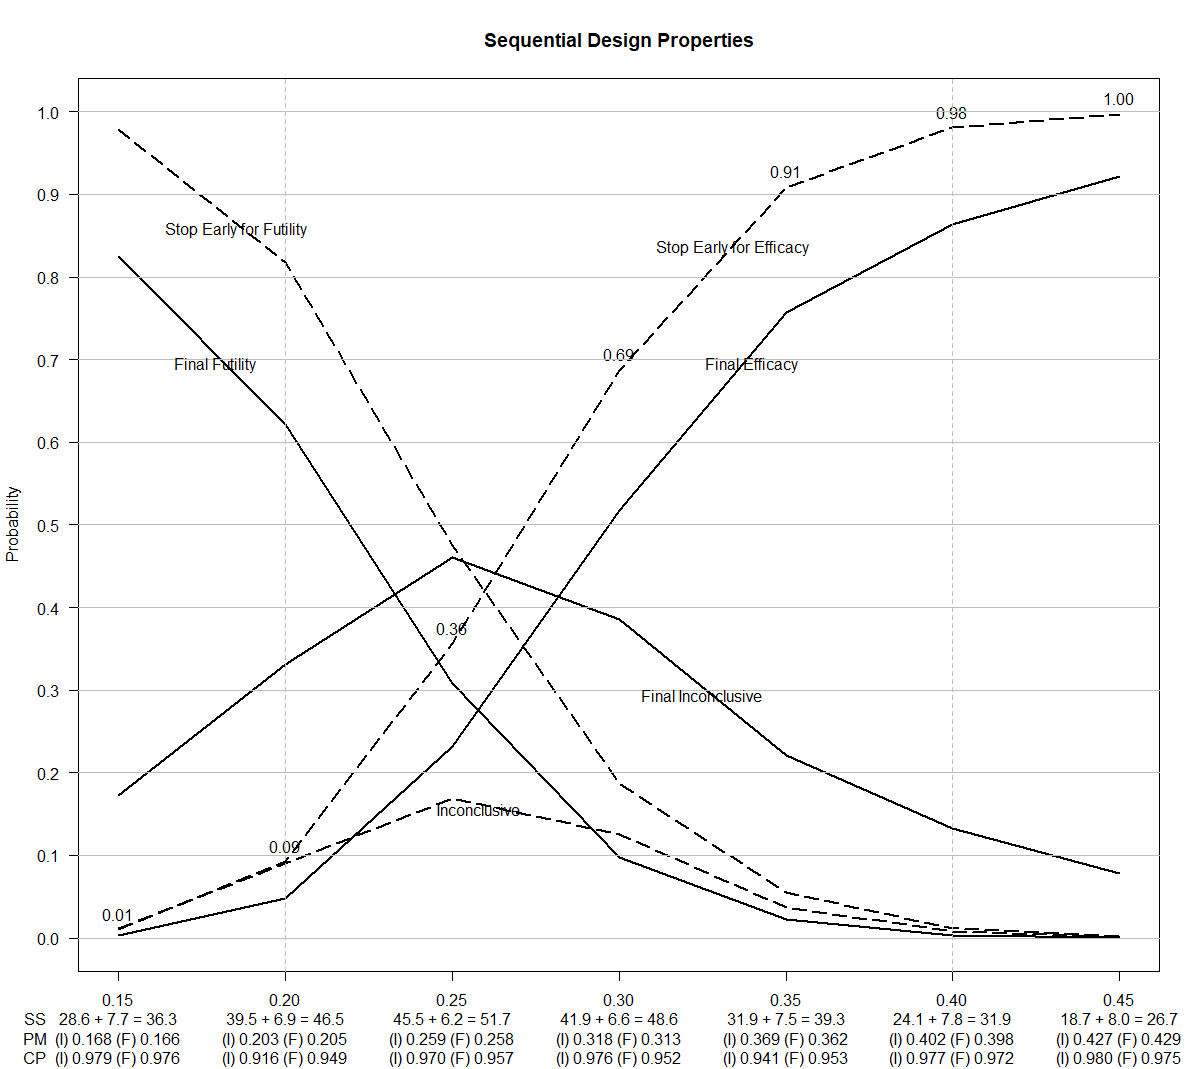
\includegraphics[width=6in]{D:/Users/ekwiatko/Documents/GitHub/Bayesian-Sequential-Monitoring/00-paper/FIGURES/sequential_design_properties_2}
%\caption{Shows agreement between sequential and final determinations as they relate to the strict cut-offs}
%\end{figure}
%\newpage
\subsubsection{Type 1 error rate by the frequency of data monitoring}
As expected, the probability of stopping enrollment due to a promising interim trial result and the Type 1 error rate at the final analysis increase with the frequency of interim monitoring, however, the increase is very slight at the final analysis. Regardless of frequency of monitoring there are good Type 1 error rates. Even at the extreme case where an interim analysis is conducted after every outcome, the probability of stopping at the interim due to a promising result when the true response is at the null level is only $0.108$ (about double the nominal rate), and even in this situation the Type 1 error rate once follow-up is complete does not exceed $0.05$. Thus Bayesian sequential monitoring has good frequentist properties even with frequent interim analyses.
%\begin{itemize}
%\item The two sides of the discussion: first is what happens during the trial regarding sequential monitoring, such as \% of time stopping early vs. trial done to completion and expected sample size. Second is the final determination of efficacy or futility and how that relates to Type 1 Error and power. 
%\item  Remember the best case for sequential monitoring is slow enrollment relative to outcome ascertainment. Slow enrollment means there is a benefit to ending trial early and reach a conclusion faster. Outcome ascertainment needs to be somewhat fast to ensure a good \# of outcomes are generated.
%\end{itemize}
%\begin{itemize}
%\item Want to highlight that the ultimate inference will have no Type 1 error inflation. At this point the ultimate inference for efficacy is still made with skeptical prior.
%\item Label lines nicely.
%\item ``Only bad thing to do is to stop learning"
%\item Enrollment rate and \% of ongoing data as operating characteristics are interesting ideas, but focus on the plots already created.
%\item Mat: Scaling on \# of subjects in each interim analysis rather than \# of interim analyses (e.g. flip X axis). Make labels go vertical or diagonal.
%\end{itemize}
\begin{figure}
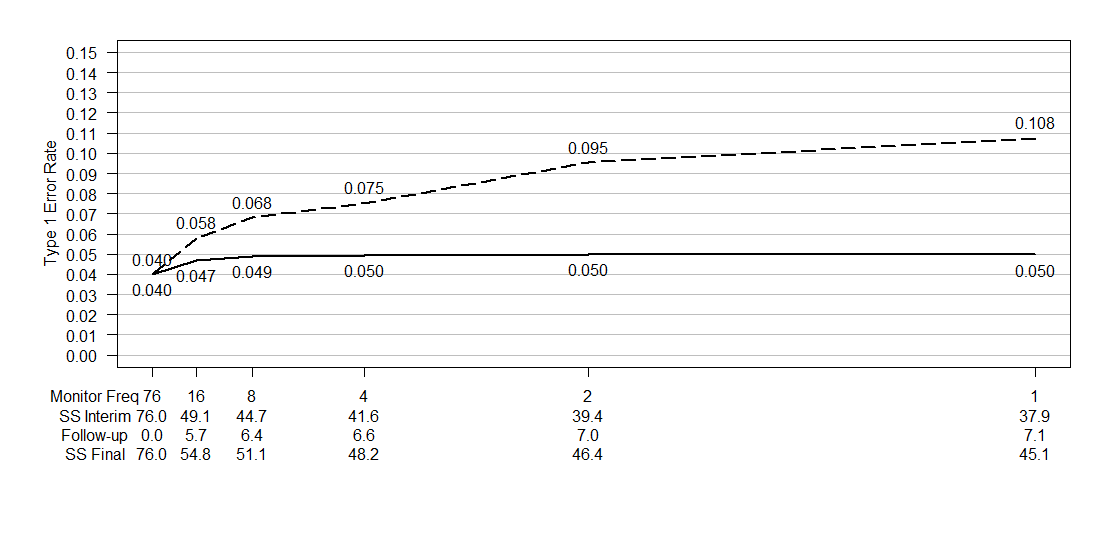
\includegraphics[width=7in]{D:/Users/ekwiatko/Documents/GitHub/Bayesian-Sequential-Monitoring/00-paper/FIGURES/type1error_0904.png}
\caption{Type 1 error rate depending on frequency of sequential monitoring}
\end{figure}

\newpage
\subsubsection{Type 1 error rate depending on enrollment schemes}
Consider the same trial but with a longer follow-up length of 8 months rather than 4 months. 
\begin{center}
\textbf{Comparision of Efficacy Stopping, Type 1 Error Rate, and Sample Size by follow-up length and frequency of sequential monitoring}
\begin{tabular}{l | cccccccc}
Mon Freq  & Eff. Stopping	&		&	T1E Final	&		&	SS Final	&		&	\% Ongoing	&\\
	&	4 mon	&	8 mon	&	4 mon	&	8 mon	&	4 mon	&	8 mon	&	4 mon	&	8 mon	\\
\hline
76	&	0.040	&	0.039	&	0.040	&	0.039	&	76.0	&	76.0	&	0.0\%	&	0.0\%	\\
16	&	0.058	&	0.056	&	0.047	&	0.042	&	54.8	&	60.0	&	10.4\%	&	18.1\%	\\
8	&	0.068	&	0.067	&	0.049	&	0.043	&	51.1	&	56.7	&	12.5\%	&	21.3\%	\\
4	&	0.075	&	0.075	&	0.050	&	0.043	&	48.2	&	54.1	&	13.7\%	&	23.4\%	\\
2	&	0.095	&	0.094	&	0.050	&	0.043	&	46.4	&	52.8	&	15.1\%	&	25.5\%	\\
1	&	0.108	&	0.107	&	0.050	&	0.043	&	45.1	&	51.7	&	15.7\%	&	26.8\%	
\end{tabular}
\end{center}
Note that the probability of efficacy stopping and Type 1 error rate increase monotonically for both specifications of follow-up length. The Type 1 error rate is lower for the 8-month follow-up design since there are more subjects in the final sample size.
%\begin{figure}
%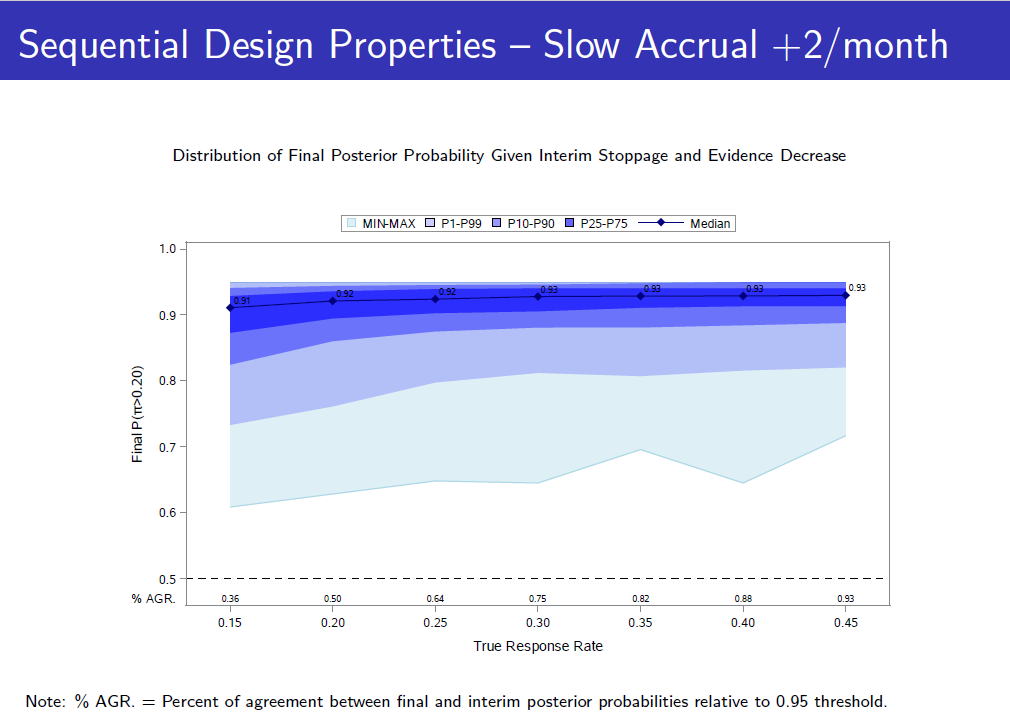
\includegraphics[width=6in]{D:/Users/ekwiatko/Documents/GitHub/Bayesian-Sequential-Monitoring/00-paper/FIGURES/evidence_decrease.png}
%\caption{Have the necessary data summaries in R, just need to replicate the plot.}
%\end{figure}

%The inference priors will be of the form $\pi_{I}=\omega\cdot\pi_{S}+(1-\omega)\cdot\pi_E$ with $\omega\in\{0,1/4,1/2,3/4,1\}$.
%\begin{center}
%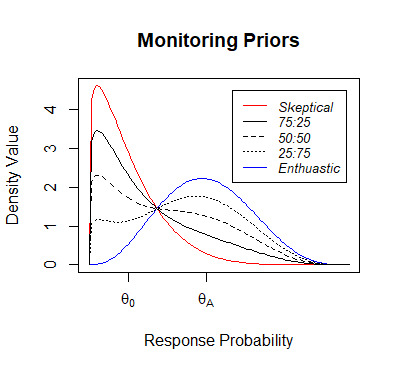
\includegraphics[width=5in]{D:/Users/ekwiatko/Documents/GitHub/Bayesian-Sequential-Monitoring/00-paper/FIGURES/figure3_2.png}
%\end{center}

%\begin{center}
%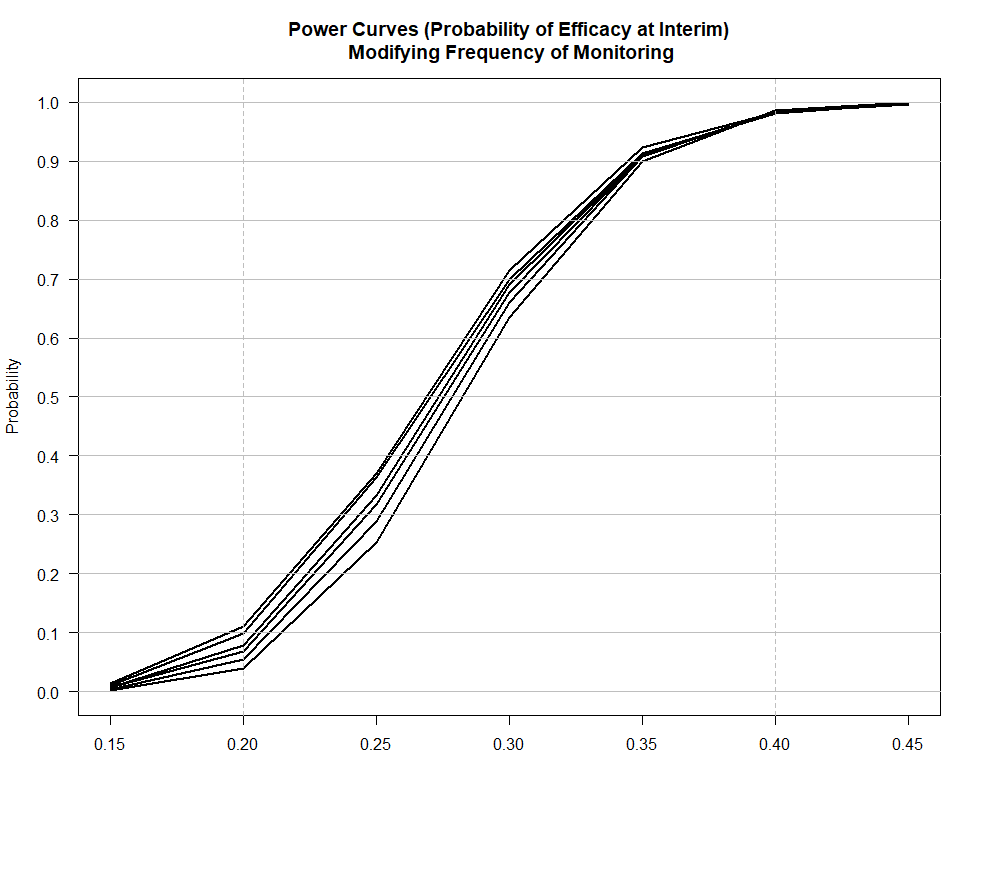
\includegraphics[width=3in]{D:/Users/ekwiatko/Documents/GitHub/Bayesian-Sequential-Monitoring/00-paper/FIGURES/power_curves}
%\end{center}
\newpage
\section{Robustness of parameterizations of monitoring priors}
The spike-slab and flattened priors are both 2-part mixtures of Beta distributions.
\begin{itemize}
\item Test the hypothesis that power curves will be identical and what will change is the expected sample sizes and that varying the decay rate will affect bias not Type I/II error
\item Actually, having one prior ``default" and the other spike-slab changes the monitoring result substantially. When using the spike-slab skeptical prior and the default enthuastic prior, the determination of efficacy at the interim is made less frequently than when using the default skeptical prior. Similarly, when using the spike-slab enthuastic prior and the default skeptical prior, the determination of futility is made less frequently than when using the default enthuastic prior.
\end{itemize}
\begin{figure}
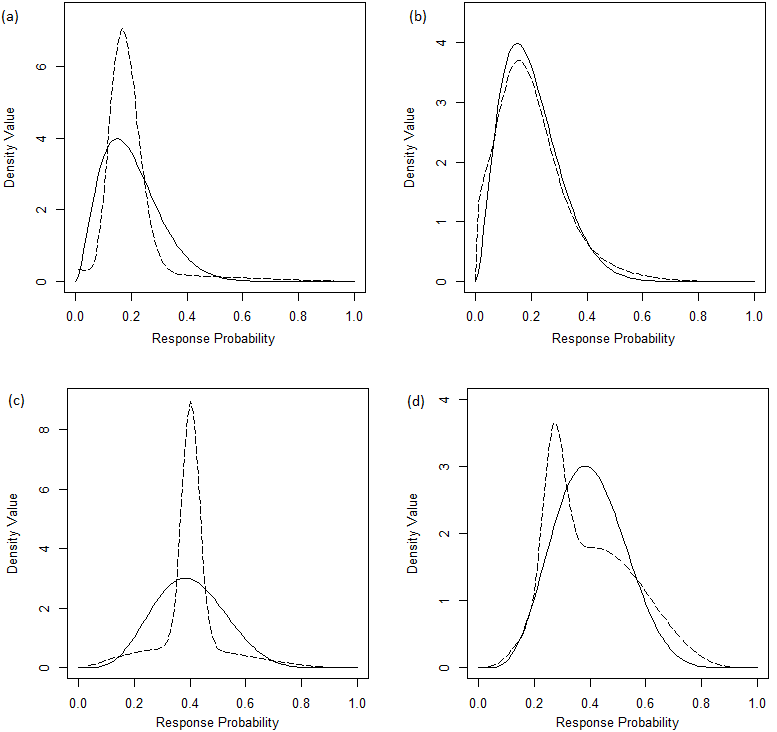
\includegraphics[width=6in]{D:/Users/ekwiatko/Documents/GitHub/Bayesian-Sequential-Monitoring/00-paper/FIGURES/figure5.png}
 \caption{(a) Spike-slab skeptical prior (b) Flattened skeptical prior (c) Spike-slab enthuastic prior (d) Flattened enthuastic prior}
\end{figure}
\begin{figure}
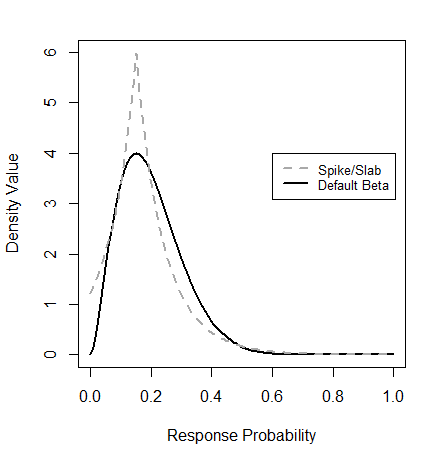
\includegraphics[width=7in]{D:/Users/ekwiatko/Documents/GitHub/Bayesian-Sequential-Monitoring/00-paper/FIGURES/spike-slab_skeptical}
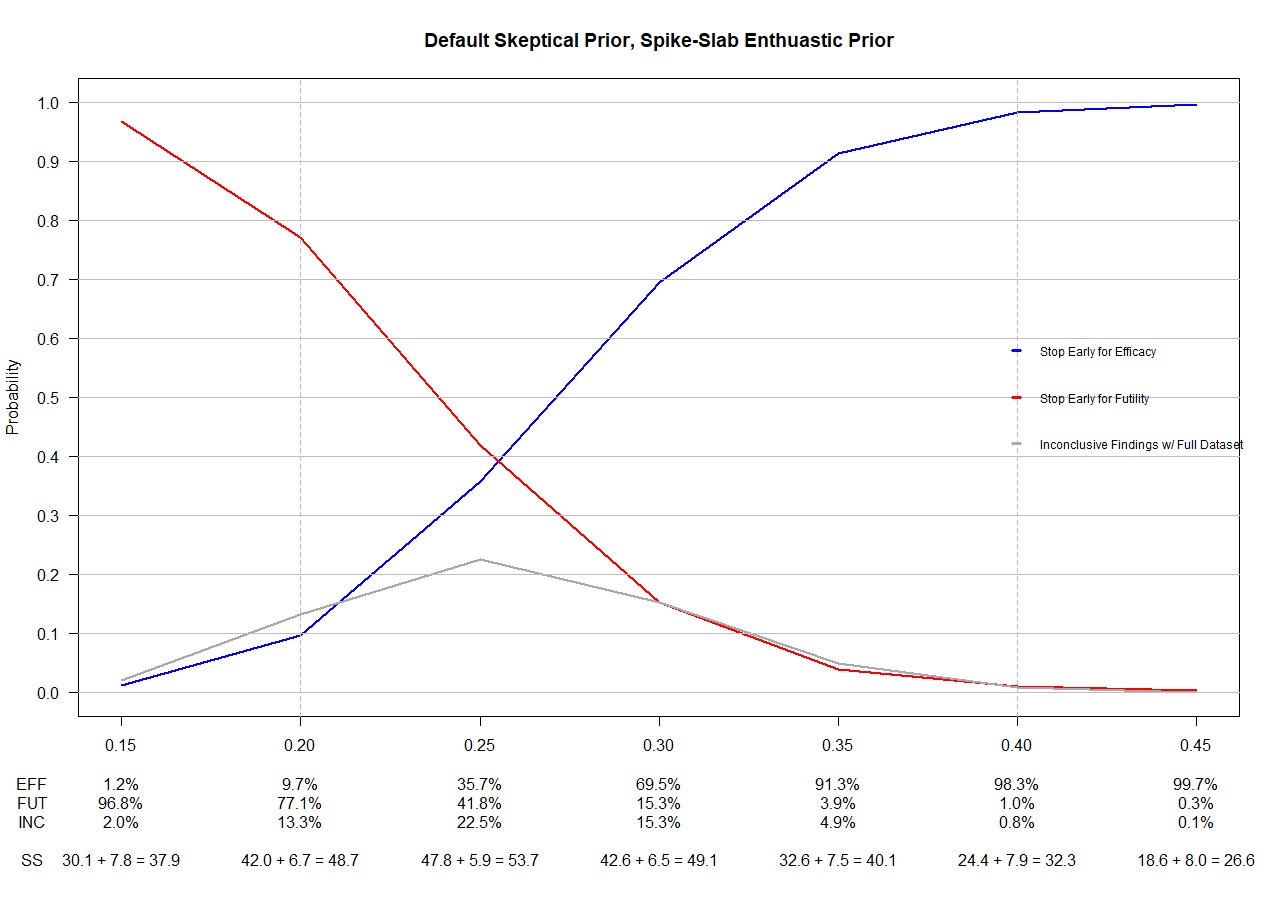
\includegraphics[width=7in]{D:/Users/ekwiatko/Documents/GitHub/Bayesian-Sequential-Monitoring/00-paper/FIGURES/spike-slab_enthuastic}
\caption{(a) Spike-slab skeptical prior and default enthuastic prior (b) Default skeptical prior and spike-slab enthuastic prior}
\end{figure}
\newpage




%\subsubsection*{Vemurafenib Trial }
%``In this study, a response rate of 15\% at week
%8 was considered to be low, a response rate of
%45\% was considered to be high, and a response
%rate of 35\% was considered to be low but still
%desirable and indicative of efficacy. Assuming
%response rates as specified in the hypothesis testing, a power of 80\% for a high response rate and
%70\% for the low but still desirable response rate,
%and a two-sided alpha level of 0.1, we calculated
%that the number of patients required in each
%cohort would be 7, 13, or 19, depending on the
%results obtained."
\subsection{Parallel Two-Group Superiority Trial /w Continuous Binary Endpoint}
Interesting because prior is on risk difference [-1,1] while also being non-informative on control group. Will need numerical integration to evalutate posteriors.
\subsection{Three-Arm, Placebo Controlled Non-Inferiority Trial w/ Continuous Endpoint}
\begin{align*}
P&\rightarrow\beta_0 \text{ (placebo)}\\
C&\rightarrow\beta_0+\beta_1 \text{ (control)}\\
A&\rightarrow\beta_0+\beta_1+\beta_2 \text{ (active)}\\
H_0&:\beta_2-\delta\beta_1\leq 0
\end{align*}
Parameters of interest $(\beta_1,\beta_2)$, nuisance parameters $(\beta_0,\sigma^2)$.

Need priors $\pi(\beta_0), \pi(\beta_1), \pi(\beta_2|\beta_1)$. 

Will use MCMC to evaluate posteriors.
\section{Discussion -- (MATT/EVAN)}
Q: Why not reverse engineer priors to have exact Type 1 error properties?

A: This would basically be a frequentist method, in that the design would have to be adhered to exactly (including number and timing of data monitoring). Philosophically, designing a Bayesian study that requires rigid monitoring rules loses the advantages of Bayes from the likelihood principle.
%\section{Example of Parallel Two-Group Design}
%
%In this section we consider a sequential monitoring approach in a parallel two-group setting using a binary response endpoint.
%
%We consider the case where the goal is prove superiority of an investigational product (IP) to a control 
%which could be a placebo.
%
%Let $\pi_0$ represent the response rate the control group and $\pi_1$ represent the response probability for the IP group.
%
%Here we wish to elicit pessimistic and enthusiastic priors consistent with the following:
% \begin{enumerate}
%  \item The control group response probability is expected to be approximately $0.20$ and investigators are relatively sure
%		    that the it will be between 0.5 and 0.35.
%				
%	\item The IP group response probability is likely to provide an improvement of approximately 0.20.
%\end{enumerate}
%
%In this setting pessimism or optimism is reflected in the induced prior on the difference in proportions $\pi_1 - \pi_0$.
%
%One easy way to specify such a prior in this case is to elicit a bivariate normal prior for $\pi_0$ and $\pi_1$ truncated to the unit square.  


%
%		\begin{figure}
%      \centering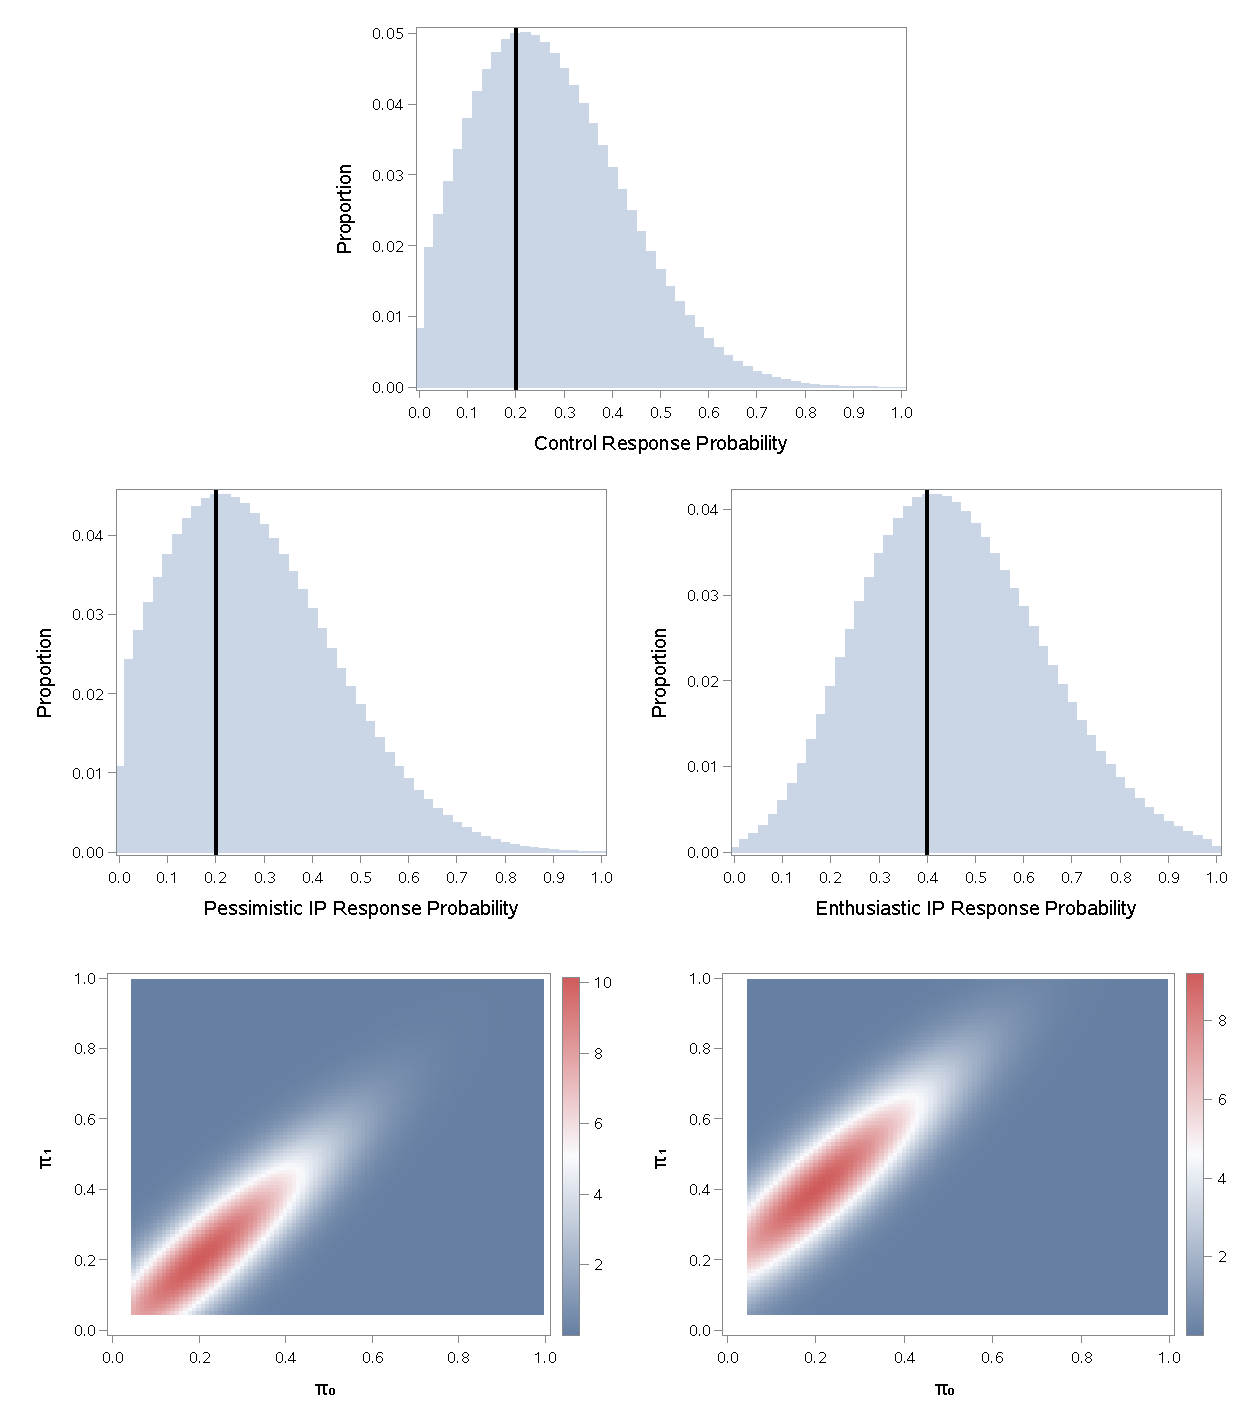
\includegraphics[scale=0.70]{./FIGURES/BINARY-PRIORS.pdf}
%      \caption{Prior for Control Group Response Probability \label{fig:pmp}}
%    \end{figure}
			


%\bigskip
\newpage
\begin{center}
{\large\bf SUPPLEMENTARY MATERIAL}
\end{center}
\section{Beta Priors}
Beta priors for $\theta$ will be used to provide closed-form expressions of the posterior distributions via Beta-Binomial conjugacy (the posterior distribution $p(\theta|\mathbf{D})$ will be Beta distributed). The Beta distribution has two shape parameters. These parameters can be determined uniquely by specifying the desired mean and variance of the distribution.  The variance for the skeptical and enthuastic priors is then uniquely determined through by the choice of threshold $\delta$. In particular, let $\pi_S(\theta)\sim \mathcal{B}(\alpha,\beta)$ be Beta distributed with shape parameters $(\alpha,\beta)$. There is a single choice of $(\alpha,\beta)$ such that:
\begin{align*}
\theta_0=E(\pi_S)=\int_{\Theta}\pi_S(\theta)d\theta=\frac{\alpha}{\alpha+\beta}\text{ and }\delta=\int_{\Theta_0}\pi_S(\theta)d\theta=\int_{0}^{\theta_0}\frac{\theta^{\alpha-1}(1-\theta)^{\beta-1}}{B(\alpha,\beta)}d\theta
\end{align*}
where $B(\alpha,\beta)$ is the Beta function.

Alternatively, the variance could be determined by specifying a desired quantile of the prior distribution which would then be reflected in $\delta$.  Then there is a single choice of $(\alpha,\beta)$ such that
\begin{align*}
\theta_0=E(\pi_S)=\int_{\Theta}\pi_S(\theta)d\theta=\frac{\alpha}{\alpha+\beta}\text{ and }\lambda=\int_{\theta_A}^{1}\pi_S(\theta)d\theta=\int_{\theta_A}^{1}\frac{\theta^{\alpha-1}(1-\theta)^{\beta-1}}{B(\alpha,\beta)}d\theta,
\end{align*}
in which case $\delta=\int_{\Theta_0}\pi_S(\theta)d\theta$ is a deterministic quantity.
%\begin{center}
%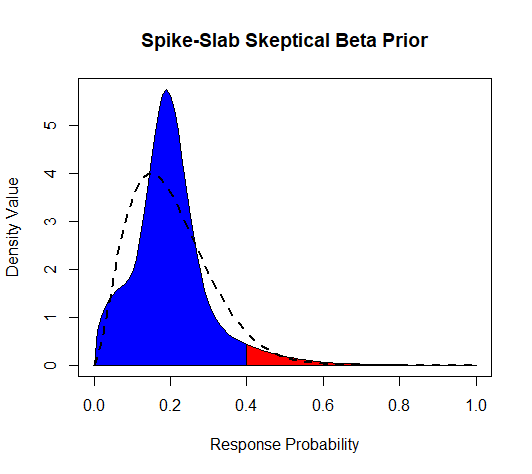
\includegraphics[width=5in]{D:/Users/ekwiatko/Documents/GitHub/Bayesian-Sequential-Monitoring/00-paper/FIGURES/ss_skpt}
%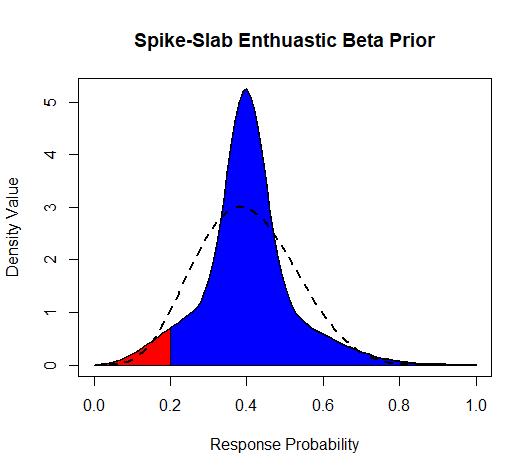
\includegraphics[width=5in]{D:/Users/ekwiatko/Documents/GitHub/Bayesian-Sequential-Monitoring/00-paper/FIGURES/ss_enth}
%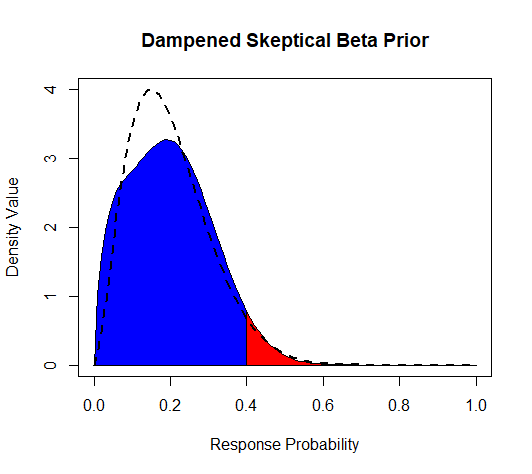
\includegraphics[width=5in]{D:/Users/ekwiatko/Documents/GitHub/Bayesian-Sequential-Monitoring/00-paper/FIGURES/damp_skpt}
%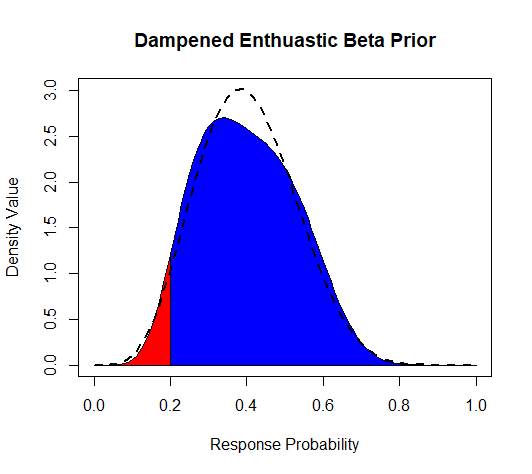
\includegraphics[width=5in]{D:/Users/ekwiatko/Documents/GitHub/Bayesian-Sequential-Monitoring/00-paper/FIGURES/damp_enth}
%\end{center}
\section{BibTeX}

 \bibliographystyle{agsm}
 \bibliography{./References}		

\end{document}
